%% chapter12_slides.tex
%% Chapter 12: Infimal Convolution
%% Bauschke & Combettes --- Convex Analysis and Monotone Operator Theory
%% in Hilbert Spaces, 2nd ed. (CMS Books in Mathematics, Springer, 2017)
%% Compile: pdflatex -interaction=nonstopmode chapter12_slides.tex  (run twice)

\documentclass[aspectratio=169,10pt]{beamer}

\usetheme{Madrid}
\usecolortheme{seahorse}
\usefonttheme{professionalfonts}
\setbeamertemplate{footline}[frame number]
\setbeamertemplate{navigation symbols}{}

%% Packages
\usepackage{amsmath,amssymb,mathtools}
\usepackage{graphicx}
\usepackage{listings}
\usepackage{xcolor}
\usepackage{booktabs}
\usepackage{microtype}

\graphicspath{{figures/}}

%% Python listings style
\lstdefinestyle{python}{
  language=Python,
  basicstyle=\ttfamily\scriptsize,
  keywordstyle=\color{blue!80!black}\bfseries,
  commentstyle=\color{green!50!black}\itshape,
  stringstyle=\color{orange!80!black},
  numbers=left,
  numberstyle=\tiny\color{gray},
  stepnumber=1,
  numbersep=4pt,
  frame=single,
  backgroundcolor=\color{gray!7},
  breaklines=true,
  showstringspaces=false,
  tabsize=4,
  captionpos=b,
}

%% Maths shortcuts
\newcommand{\cH}{\mathcal{H}}
\newcommand{\cK}{\mathcal{K}}
\newcommand{\R}{\mathbb{R}}
\newcommand{\N}{\mathbb{N}}
\newcommand{\norm}[1]{\left\|#1\right\|}
\newcommand{\inner}[2]{\left\langle #1 \mid #2 \right\rangle}
\newcommand{\dom}{\operatorname{dom}}
\newcommand{\epi}{\operatorname{epi}}
\newcommand{\Argmin}{\operatorname{Argmin}}
\newcommand{\Fix}{\operatorname{Fix}}
\newcommand{\Prox}{\operatorname{Prox}}
\newcommand{\co}{\square}
\newcommand{\me}[1]{{}^{#1}\!f}
\newcommand{\megamma}{{}^{\gamma}\!f}

%% Title info
\title[Convex Analysis \& MOT -- Ch.12]{Convex Analysis and Monotone Operator Theory in Hilbert Spaces}
\subtitle{Chapter 12: Infimal Convolution}
\author{Based on Bauschke \& Combettes}
\institute{CMS Books in Mathematics, Springer, 2nd ed., 2017}
\date{}

% ---------------------------------------------------------------
\begin{document}
% ---------------------------------------------------------------

\begin{frame}
  \titlepage
\end{frame}

\begin{frame}{Chapter Outline}
  \tableofcontents
\end{frame}

% =================================================================
\section{Definition and Basic Facts}
% =================================================================

\begin{frame}[allowframebreaks]{Notation You'll Need}

  Throughout, $\cH$, $\cK$ are real Hilbert spaces with inner product
  $\inner{\cdot}{\cdot}$ and induced norm $\norm{\cdot}$.

  \begin{itemize}
    \item $\Gamma_0(\cH)$: proper, lower semicontinuous, convex functions
      $\cH\to\left]-\infty,+\infty\right]$.
    \item $\dom f=\{x\in\cH: f(x)<+\infty\}$; $f$ \textbf{proper} if
      $\dom f\ne\varnothing$ and never takes value $-\infty$.
    \item $\epi f=\{(x,\xi)\in\cH\times\R: f(x)\le\xi\}$, the \textbf{epigraph}.
    \item $\iota_C$: \textbf{indicator function} ($0$ on $C$, $+\infty$ off $C$).
    \item $d_C(x)=\inf_{y\in C}\norm{x-y}$: \textbf{distance} to $C$;
      $P_C$: \textbf{projection} onto closed convex $C$.
    \item $\tau_y f = f(\cdot - y)$: \textbf{translation} by $y$.
    \item $f^*$: the \textbf{conjugate} (Fenchel transform) of $f$.
  \end{itemize}

  \framebreak

  Key convention: Throughout, we write $\inf_{y \in \cH}$ to mean the
  infimum is taken over the entire Hilbert space $\cH$.

\end{frame}

\begin{frame}[allowframebreaks]{Definition 12.1: Infimal Convolution}

  \textbf{Definition 12.1} -- For $f, g: \cH \to \left]-\infty, +\infty\right]$:

  The \textit{infimal convolution} (or epigraphical sum) is
  \begin{equation}
    (f \co g): \cH \to \left]-\infty, +\infty\right] : x \mapsto \inf_{y \in \cH} \left( f(y) + g(x-y) \right)
  \end{equation}

  \begin{itemize}
    \item $(f \co g)(x)$ is \textbf{exact at} $x$ if the infimum is
      \textbf{attained} ($\exists y$ achieving the minimum).
    \item $(f \co g)$ is \textbf{exact} if exact at every point in its domain.
    \item When exact, we write $f \overline{\co} g$.
  \end{itemize}

  \framebreak

  \textbf{Key Properties from Definition:}

  \begin{enumerate}
    \item[(i)] \textbf{Domain:}
    \[
      \dom(f \co g) = \dom f + \dom g = \{ x + y : x \in \dom f, y \in \dom g \}
    \]

    \item[(ii)] \textbf{Epigraph relation:}
    \[
      \epi(f \co g) = \{ (x, \xi_1 + \xi_2) : x = y + z, (y,\xi_1) \in \epi f, (z,\xi_2) \in \epi g \}
    \]

    \item[(iii)] \textbf{Commutative:} $f \co g = g \co f$ (when both sides defined).

    \item[(iv)] \textbf{Associative:} $(f \co g) \co h = f \co (g \co h)$.
  \end{enumerate}

\end{frame}

\begin{frame}{Example 12.2: Infimal Convolution of Indicator Functions}

  \textbf{Example 12.2} -- Let $C, D \subseteq \cH$ be nonempty closed convex sets.

  Then:
  \[
    (\iota_C \co \iota_D)(x) = \iota_{C+D}(x) = \begin{cases}
      0 & \text{if } x \in C + D \\
      +\infty & \text{otherwise}
    \end{cases}
  \]

  \vspace{0.3cm}

  \textbf{Interpretation:} Infimal convolution of indicator functions
  yields the indicator of the Minkowski sum.

  \vspace{0.5cm}

  \textbf{General composition rule:}
  \[
    \iota_C \co f = f|_C \quad \text{and} \quad f \co \iota_C = f(-\cdot)|_{-C}
  \]

\end{frame}

\begin{frame}{Definition 12.5: Continuous Affine Minorant}

  \textbf{Definition 12.5} -- $f$ possesses a \textit{continuous affine
  minorant with slope} $u \in \cH$ if
  \[
    \langle \cdot \mid u \rangle \text{ is bounded below by } f
  \]

  That is, $\exists \eta \in \R$ such that $f(y) \geq \langle y \mid u \rangle + \eta$ for all $y \in \cH$.

  \vspace{1cm}

  \textbf{Intuition:} The linear functional with slope $u$ provides a lower bound for $f$.

  \vspace{1cm}

  \textbf{Examples:}
  \begin{itemize}
    \item If $f$ is differentiable with bounded gradient, it has a continuous
      affine minorant.
    \item The absolute value $f(x) = |x|$ has affine minorant with any $|u| \le 1$.
  \end{itemize}

\end{frame}

\begin{frame}[allowframebreaks]{Proposition 12.6: Properties with Affine Minorants}

  \textbf{Proposition 12.6} -- Suppose $f, g, h: \cH \to \left]-\infty, +\infty\right]$ and $u \in \cH$.

  \textbf{(i)} If $f$ and $g$ possess continuous affine minorants with slope
  $u$, then $f \co g$ possesses such a minorant, and $-\infty \notin (f \co g)(\cH)$.

  \vspace{0.3cm}

  \textbf{(ii)} $\dom(f \co g) = \dom f + \dom g$.

  \vspace{0.3cm}

  \textbf{(iii)} $f \co g = g \co f$ (commutativity).

  \vspace{0.3cm}

  \textbf{(iv)} Suppose $f, g, h$ all possess affine minorants with the same
  slope. Then $(f \co g) \co h = f \co (g \co h)$ (associativity).

  \framebreak

  \textbf{Key Formula:} From the definition,
  \[
    (f \co g)(x) = \inf_{(y,z) \in \cH \times \cH, \, y+z=x} \left( f(y) + g(z) \right)
  \]

  \vspace{0.5cm}

  \textbf{Remark 12.7:} The conditions on affine minorants are essential.
  Without them, pathological behavior can occur (e.g., $g \equiv -\infty$).

\end{frame}

\begin{frame}{Proposition 12.8: Epigraph and Exactness}

  \textbf{Proposition 12.8} -- For functions $f, g: \cH \to \left]-\infty, +\infty\right]$:

  \begin{enumerate}
    \item[(i)] $\epi f + \epi g \subseteq \epi(f \co g)$.
    \item[(ii)] If $f \co g = f \overline{\co} g$ (is exact), then
      \[
        \epi f + \epi g = \epi(f \co g)
      \]
  \end{enumerate}

  \vspace{1cm}

  \textbf{Interpretation:} The epigraph of an infimal convolution contains the
  Minkowski sum of the epigraphs. Equality holds precisely when the
  infimal convolution is exact.

  \vspace{0.5cm}

  \textbf{Impact:} This connects the algebraic operation (infimal convolution)
  to geometric properties (epigraphs and their sums).

\end{frame}

\begin{frame}{Proposition 12.9: Infimal Convolution with Power of Norm}

  \textbf{Proposition 12.9} -- Let $f$ be proper, $p \in [1, +\infty[$, and define
  \[
    g_\gamma = f \co \left( \frac{1}{\gamma p} \norm{\cdot}^p \right)
  \]

  Then for all $\gamma \in \R_{++}$:

  \begin{enumerate}
    \item[(i)] $\dom g_\gamma = \cH$.
    \item[(ii)] $\inf f(\cH) \le g_\gamma(x) \le g_\mu(x) \le f(x)$ when $0 < \gamma < \mu$.
    \item[(iii)] $\inf g_\gamma(\cH) = \inf f(\cH)$.
    \item[(iv)] $g_\gamma(x) \downarrow \inf f(\cH)$ as $\gamma \to +\infty$.
    \item[(v)] $g_\gamma$ is bounded above on every ball in $\cH$.
  \end{enumerate}

  \vspace{0.5cm}

  \textbf{Formula:}
  \[
    g_\gamma(x) = \inf_{y \in \cH} \left( f(y) + \frac{1}{\gamma p} \norm{x - y}^p \right)
  \]

\end{frame}

% =================================================================
\section{Infimal Convolution of Convex Functions}
% =================================================================

\begin{frame}{Proposition 12.11: Infimal Convolution of Convex Functions}

  \textbf{Proposition 12.11} -- If $f$ and $g$ are convex functions from
  $\cH$ to $\left]-\infty, +\infty\right]$, then $f \co g$ is convex.

  \vspace{1cm}

  \textbf{Proof outline:} Define the marginal function
  \[
    F: \cH \times \cH \to \left]-\infty, +\infty\right], \quad F(y,z) = f(y) + g(z)
  \]

  $F$ is convex (product of convex functions). The infimal convolution
  corresponds to the marginal function
  \[
    (f \co g)(x) = \inf_{y+z=x} F(y,z)
  \]

  By Proposition 8.35, the marginal of a convex function is convex. $\square$

  \vspace{1cm}

  \textbf{Key consequence:} Many important functions (Moreau envelope,
  distance to convex set, etc.) inherit convexity via infimal convolution.

\end{frame}

\begin{frame}{Corollary 12.12: Distance Function to Convex Set}

  \textbf{Corollary 12.12} -- Let $C$ be a convex subset of $\cH$. Then
  the distance function
  \[
    d_C(x) = \inf_{y \in C} \norm{x - y}
  \]

  is convex.

  \vspace{1cm}

  \textbf{Proof:} By Example 12.2,
  \[
    d_C = \iota_C \co \norm{\cdot}
  \]

  Both $\iota_C$ and $\norm{\cdot}$ are convex, so their infimal
  convolution is convex. $\square$

  \vspace{1cm}

  \textbf{Remark:} This is a powerful tool: convexity of the distance
  function ensures nice properties in optimization.

\end{frame}

\begin{frame}[allowframebreaks]{Proposition 12.14: Exactness for Convex Functions}

  \textbf{Proposition 12.14} -- Let $f, g \in \Gamma_0(\cH)$, and suppose one:

  \begin{enumerate}
    \item[(i)] $f$ is \textbf{supercoercive}, or
    \item[(ii)] $f$ is \textbf{coercive} and $g$ is \textbf{bounded below}
  \end{enumerate}

  Then $f \co g = f \overline{\co} g \in \Gamma_0(\cH)$, i.e., the infimal
  convolution is exact and returns to $\Gamma_0$.

  \vspace{1cm}

  \textbf{Key idea of proof:}

  If $(x_n) \to x$ and $(f \co g)(x_n) \to \mu$, then there exist
  minimizers $y_n$ such that $f(y_n) + g(x_n - y_n) = (f \co g)(x_n)$.

  By supercoercivity or coercivity, $(y_n)$ remains bounded. Passing
  to a subsequence and using lower semicontinuity shows
  \[
    (f \co g)(x) \le \liminf_{n} (f \co g)(x_n) = \mu
  \]

  Thus, $f \co g$ is sequentially lower semicontinuous.

  \framebreak

  \textbf{Consequence:} Under mild conditions, the infimal convolution of
  two proper convex lsc functions is again proper convex lsc.

\end{frame}

% =================================================================
\section{Moreau Envelope and Proximity Operator}
% =================================================================

\begin{frame}{Definition 12.20: Moreau Envelope}

  \textbf{Definition 12.20} -- Let $f: \cH \to \left]-\infty, +\infty\right]$
  and $\gamma \in \R_{++}$.

  The \textit{Moreau envelope} of $f$ with parameter $\gamma$ is:
  \begin{align}
    \me{\gamma} &= f \co \left( \frac{1}{2\gamma} \norm{\cdot}^2 \right) \\
    &: \cH \to \left]-\infty, +\infty\right] \\
    &: x \mapsto \inf_{y \in \cH} \left( f(y) + \frac{1}{2\gamma} \norm{x - y}^2 \right)
  \end{align}

  \vspace{0.5cm}

  \textbf{Alternative notation:} $f_\gamma$, $J_\gamma f$, $M_\gamma f$.

  \vspace{0.5cm}

  \textbf{Example 12.21:} For a convex set $C$,
  \[
    \me{\gamma} \iota_C = \frac{1}{2\gamma} d_C^2
  \]

  The Moreau envelope of an indicator is the (normalized) squared distance.

\end{frame}

\begin{frame}[fragile]{Figure: Moreau Envelope}

  \centering
  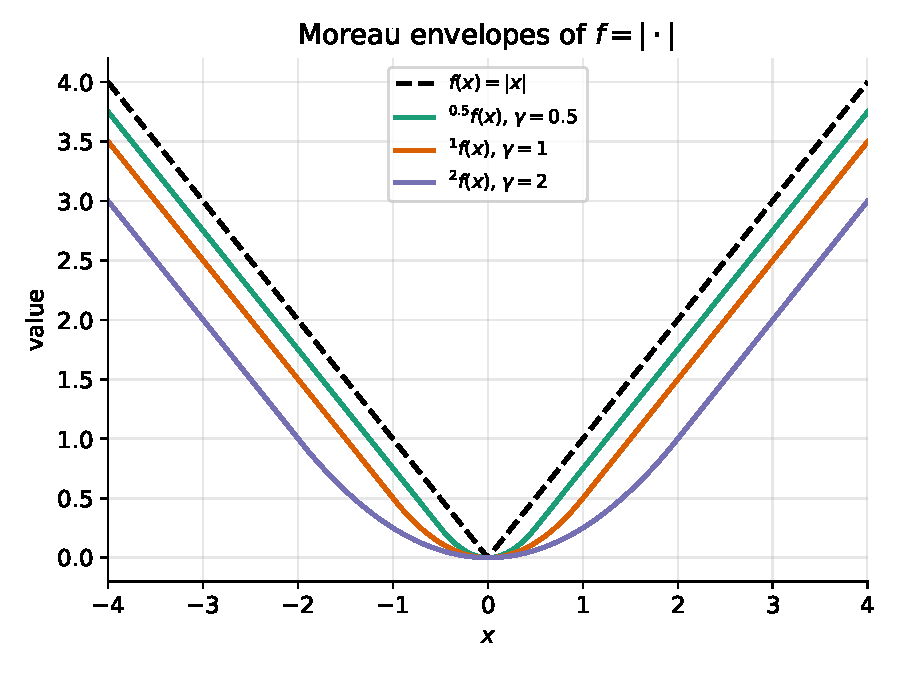
\includegraphics[width=0.85\textwidth]{fig_moreau_envelope.pdf}

\end{frame}

\begin{frame}[allowframebreaks]{Proposition 12.22: Composition Property}

  \textbf{Proposition 12.22} -- For $\gamma, \mu \in \R_{++}$:

  \begin{enumerate}
    \item[(i)] $\mu(\me{\gamma}) = \me{\gamma}(\me{\mu})$.
    \item[(ii)] $\me{\gamma}(\me{\mu}) = \me{\gamma + \mu}$.
  \end{enumerate}

  \vspace{0.5cm}

  \textbf{Proof of (ii):} Unfold the definitions:
  \begin{align}
    \me{\gamma}(\me{\mu})
    &= \left( f \co \frac{1}{2\mu}\norm{\cdot}^2 \right) \co \frac{1}{2\gamma}\norm{\cdot}^2 \\
    &= f \co \left( \frac{1}{2\mu}\norm{\cdot}^2 \co \frac{1}{2\gamma}\norm{\cdot}^2 \right) \\
    &= f \co \frac{1}{2(\gamma+\mu)} \norm{\cdot}^2 \\
    &= \me{\gamma + \mu}
  \end{align}

  The middle step uses a classical identity on composition of the
  squared-norm function.

  \framebreak

  \textbf{Significance:} The Moreau envelope is stable under composition. Applying the Moreau envelope multiple times with parameters $\gamma_1, \gamma_2$ is equivalent to applying once with $\gamma_1 + \gamma_2$.

\end{frame}

\begin{frame}{Proposition 12.30: Differentiability of Moreau Envelope}

  \textbf{Proposition 12.30} -- Let $f \in \Gamma_0(\cH)$ and $\gamma \in \R_{++}$.
  Then $\me{\gamma}: \cH \to \R$ is Fréchet differentiable on $\cH$, with gradient
  \[
    \nabla(\me{\gamma}) = \gamma^{-1} (\text{Id} - \Prox_{\gamma f})
  \]

  where $\Prox_{\gamma f}$ is the proximity operator (see next).

  Moreover, $\nabla(\me{\gamma})$ is $\gamma^{-1}$-Lipschitz continuous.

  \vspace{1cm}

  \textbf{Key implication:} The Moreau envelope provides a smooth
  approximation to a non-smooth function $f$.

  \vspace{0.5cm}

  \textbf{Application:} In optimization, one can use smooth gradient
  methods on $\me{\gamma}$ instead of non-smooth algorithms on $f$.

\end{frame}

\begin{frame}{Definition 12.23: Proximity Operator}

  \textbf{Definition 12.23} -- Let $f: \cH \to \left]-\infty, +\infty\right]$ and $x \in \cH$.

  The unique point $p \in \cH$ satisfying
  \[
    \me{1}(x) = \min_{y \in \cH} \left( f(y) + \frac{1}{2} \norm{x - y}^2 \right) = f(p) + \frac{1}{2} \norm{x - p}^2
  \]

  is called the \textit{proximity operator} or \textit{proximal mapping} of $f$ at $x$:
  \[
    p = \Prox_f(x)
  \]

  \vspace{1cm}

  \textbf{Alternative notation:} $\text{prox}_f(x)$, $J_f(x)$.

  \vspace{0.5cm}

  \textbf{Optimality condition:}
  \[
    x - \Prox_f(x) \in \partial f(\Prox_f(x))
  \]

  (See Chapter 14 on subdifferentials.)

\end{frame}

\begin{frame}[allowframebreaks]{Proposition 12.26: Characterization}

  \textbf{Proposition 12.26} -- Let $f \in \Gamma_0(\cH)$. Then $p = \Prox_f(x)$
  if and only if
  \[
    \forall y \in \cH, \quad \langle y - p \mid x - p \rangle + f(p) \le f(y)
  \]

  \vspace{1cm}

  \textbf{Interpretation:} This is a variational characterization: $p$ is
  the point that minimizes $y \mapsto f(y) + \frac{1}{2}\norm{x - y}^2$,
  and the above inequality captures the first-order optimality.

  \framebreak

  \textbf{Remark 12.24:} From Proposition 12.22(i), the Moreau envelope
  can be written as
  \[
    \me{\gamma}(x) = f(\Prox_{\gamma f} x) + \frac{1}{2\gamma} \norm{x - \Prox_{\gamma f} x}^2
  \]

  This shows that the Moreau envelope is determined by the proximity operator.

\end{frame}

\begin{frame}{Example 12.25: Projection onto Convex Set}

  \textbf{Example 12.25} -- If $C$ is a nonempty closed convex set, then
  \[
    \Prox_{\iota_C} = P_C
  \]

  The proximity operator of the indicator function is orthogonal projection onto $C$.

  \vspace{1cm}

  \textbf{Proof:}
  \begin{align}
    \Prox_{\iota_C}(x) &= \arg\min_{y \in \cH} \left( \iota_C(y) + \frac{1}{2} \norm{x - y}^2 \right) \\
    &= \arg\min_{y \in C} \norm{x - y}^2 \\
    &= P_C(x)
  \end{align}

  \vspace{0.5cm}

  \textbf{Consequence:} Projection is a special case of the proximity operator.

\end{frame}

\begin{frame}[fragile]{Soft-Thresholding: $\Prox_{|\cdot|}$}

  \textbf{Fundamental example:} For $f(x) = |x|$,
  \[
    \Prox_{\gamma |\cdot|}(x) = \text{sign}(x) \max(|x| - \gamma, 0)
  \]

  This is the \textbf{soft-thresholding} operator, crucial in:
  \begin{itemize}
    \item Sparse optimization and compressed sensing.
    \item $\ell^1$-regularized problems.
    \item Signal and image processing.
  \end{itemize}

  \vspace{1cm}

  \centering
  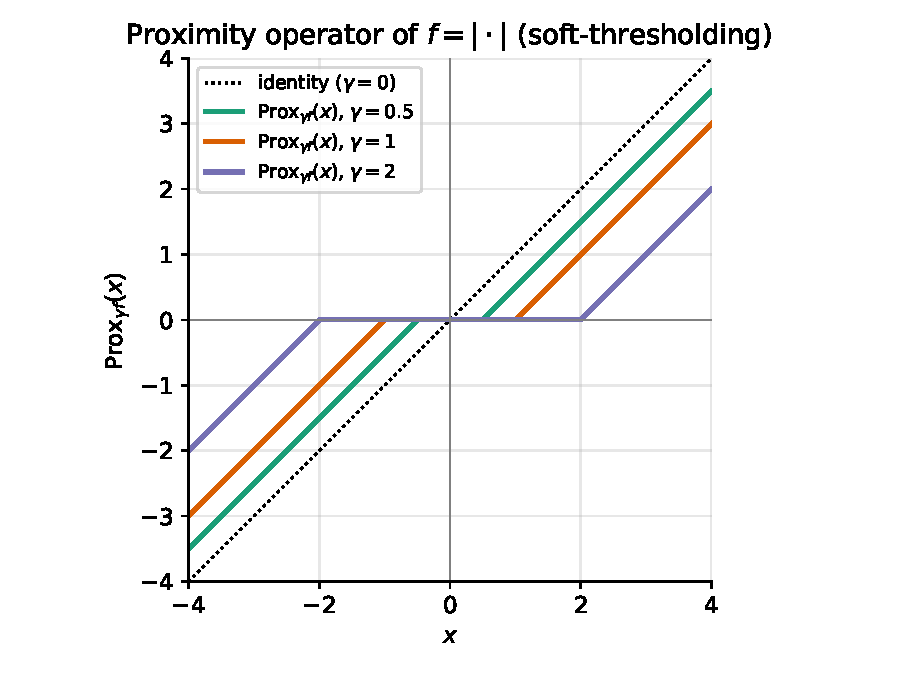
\includegraphics[width=0.8\textwidth]{fig_prox_soft_threshold.pdf}

\end{frame}

\begin{frame}[allowframebreaks]{Proposition 12.27-12.29: Nonexpansiveness and Fixed Points}

  \textbf{Proposition 12.28} -- The operators $\Prox_f$ and $\text{Id} - \Prox_f$ are
  \textit{firmly nonexpansive}:

  \begin{enumerate}
    \item[(a)] $\norm{\Prox_f x - \Prox_f y} \le \norm{x - y}$ (nonexpansive).
    \item[(b)] $\norm{\Prox_f x - \Prox_f y}^2 + \norm{(x - \Prox_f x) - (y - \Prox_f y)}^2 \le \norm{x - y}^2$.
  \end{enumerate}

  \vspace{0.5cm}

  \textbf{Proposition 12.29} -- For any $f \in \Gamma_0(\cH)$:
  \[
    \Fix(\Prox_f) = \Argmin f
  \]

  The fixed points of the proximity operator are exactly the minimizers of $f$.

  \framebreak

  \textbf{Significance for optimization:}
  \begin{itemize}
    \item Firm nonexpansiveness ensures convergence of iterative schemes.
    \item Fixed-point characterization shows that finding minimizers
      reduces to finding fixed points of $\Prox_f$.
    \item This underlies proximal gradient descent, Douglas--Rachford, ADMM, etc.
  \end{itemize}

\end{frame}

\begin{frame}{Corollary 12.31: Distance Function is Smooth}

  \textbf{Corollary 12.31} -- Let $C$ be a nonempty closed convex set.
  Then $d_C^2$ is Fréchet differentiable on $\cH$, with
  \[
    \nabla(d_C^2) = 2(\text{Id} - P_C)
  \]

  \vspace{1cm}

  \textbf{Proof:} Apply Proposition 12.30 with $f = \iota_C$ and $\gamma = 1/2$.
  By Example 12.25, $\Prox_{\iota_C} = P_C$. Thus,
  \[
    \nabla \left( \frac{1}{2} d_C^2 \right) = 2(\text{Id} - P_C) \Rightarrow
    \nabla(d_C^2) = 2(\text{Id} - P_C)
  \]

  \vspace{1cm}

  \textbf{Impact:} Squared distance to a convex set is smooth, enabling
  the use of gradient-based optimization methods.

\end{frame}

\begin{frame}[fragile]{Figure: Moreau Envelope and Proximity Operator}

  \centering
  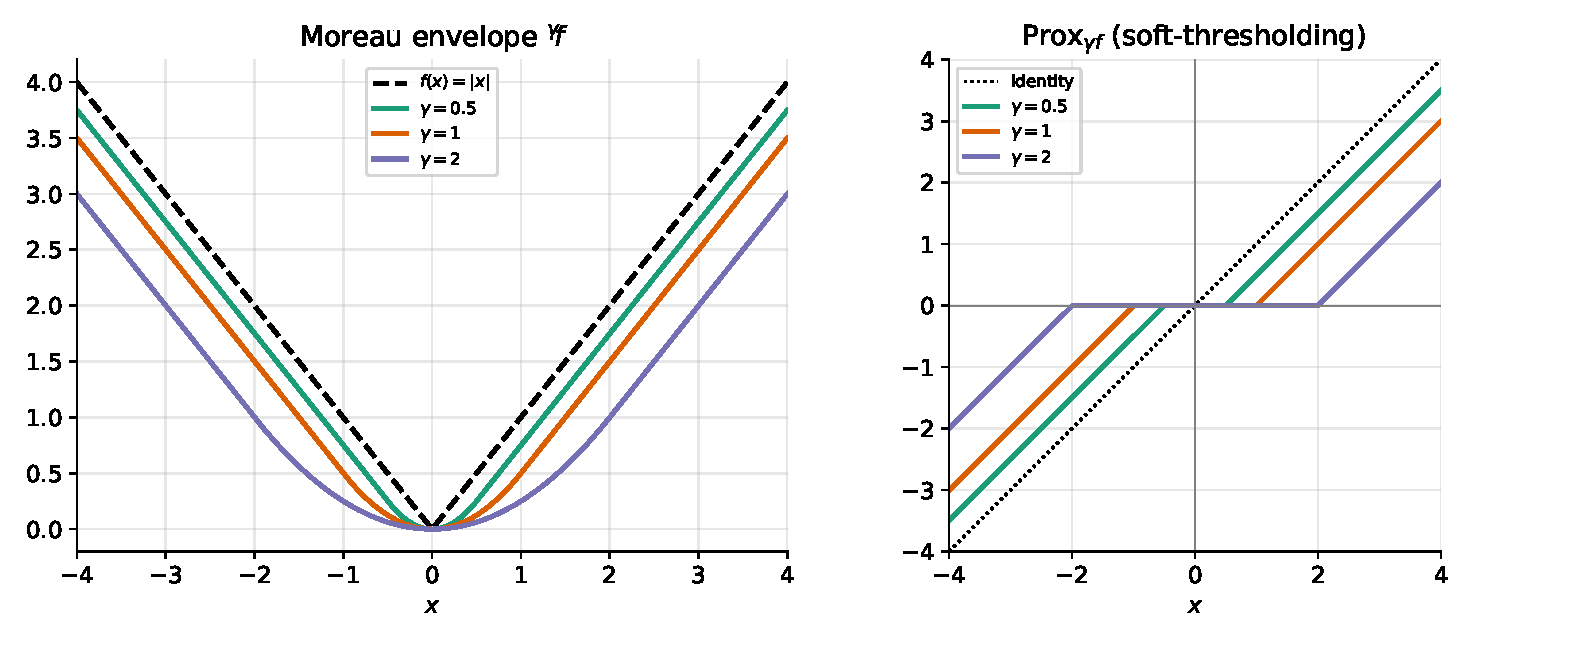
\includegraphics[width=1.0\textwidth]{fig_moreau_prox_combined.pdf}

\end{frame}

\begin{frame}{Proposition 12.33: Convergence of Sequences}

  \textbf{Proposition 12.33} -- For $f \in \Gamma_0(\cH)$ and $x \in \cH$:

  The nets $(\me{\gamma}(x))_{\gamma \in \R_{++}}$ and $(f(\Prox_{\gamma f} x))_{\gamma \in \R_{++}}$
  are decreasing with:

  \begin{enumerate}
    \item[(i)] $\me{\gamma}(x) \downarrow \inf f(\cH)$ as $\gamma \to +\infty$.
    \item[(ii)] $\me{\gamma}(x) \uparrow f(x)$ as $\gamma \downarrow 0$.
    \item[(iii)] If $x \in \dom f$, then $\me{\gamma}(x) \to f(x)$ and
      $\gamma^{-1} \norm{x - \Prox_{\gamma f} x}^2 \to 0$ as $\gamma \downarrow 0$.
  \end{enumerate}

  \vspace{1cm}

  \textbf{Interpretation:}
  \begin{itemize}
    \item As $\gamma \to 0$: Moreau envelope recovers the original function.
    \item As $\gamma \to \infty$: Envelope becomes flat, approaching the infimum.
    \item Proximity points converge to the set of minimizers.
  \end{itemize}

\end{frame}

% =================================================================
\section{Pasch--Hausdorff Envelope}
% =================================================================

\begin{frame}{Definition 12.16: Pasch--Hausdorff Envelope}

  \textbf{Definition 12.16} -- Let $f: \cH \to \left]-\infty, +\infty\right]$
  and $\beta \in \R_{++}$.

  The \textit{$\beta$-Pasch--Hausdorff envelope} of $f$ is:
  \[
    f \co (\beta \norm{\cdot})
  \]

  \vspace{1cm}

  This is the infimal convolution of $f$ with $\beta$ times the norm.

\end{frame}

\begin{frame}[allowframebreaks]{Proposition 12.17: Lipschitz Characterization}

  \textbf{Proposition 12.17} -- Let $f$ be proper, $\beta \in \R_{++}$,
  and $g = f \co (\beta \norm{\cdot})$ (the Pasch--Hausdorff envelope).
  Then exactly one holds:

  \begin{enumerate}
    \item[(i)] $f$ possesses a $\beta$-Lipschitz continuous minorant.
      In this case, $g$ is the largest such minorant.

    \item[(ii)] $f$ has no $\beta$-Lipschitz continuous minorant.
      In this case, $g \equiv -\infty$.
  \end{enumerate}

  \vspace{1cm}

  \textbf{Significance:} The Pasch--Hausdorff envelope computes the
  largest $\beta$-Lipschitz lower bound for $f$.

  \framebreak

  \textbf{Corollary 12.18} -- If $f$ is $\beta$-Lipschitz continuous, then
  \[
    f \co (\beta \norm{\cdot}) = f
  \]

  A Lipschitz function is its own envelope.

  \vspace{1cm}

  \textbf{Corollary 12.19} -- For a function $h: C \to \R$ that is
  $\beta$-Lipschitz on $C$, the function
  \[
    (f \co (\beta \norm{\cdot}))|_{\cH}
  \]

  where $f = \iota_C \vee h$ (indicator/extension), extends $h$ to
  all of $\cH$ while preserving the $\beta$-Lipschitz property.

\end{frame}

% =================================================================
\section{Infimal Postcomposition}
% =================================================================

\begin{frame}{Definition 12.34: Infimal Postcomposition}

  \textbf{Definition 12.34} -- For $f: \cH \to \left]-\infty, +\infty\right]$,
  $L: \cH \to \cK$, and $y \in \cK$:

  The \textit{infimal postcomposition} of $f$ by $L$ is:
  \[
    (L \triangleright f)(y) := \inf_{\substack{x \in \cH \\ Lx = y}} f(x)
  \]

  \vspace{1cm}

  \textbf{Compare:}
  \begin{itemize}
    \item \textbf{Infimal convolution}: $(f \co g)(x) = \inf_y [f(y) + g(x-y)]$.
    \item \textbf{Infimal postcomposition}: $(L \triangleright f)(y) = \inf_{Lx=y} f(x)$.
  \end{itemize}

  \vspace{1cm}

  $(L \triangleright f)$ is exact at $y$ if the minimum is attained.

\end{frame}

\begin{frame}[allowframebreaks]{Proposition 12.36-12.37: Properties}

  \textbf{Proposition 12.36} -- For $f: \cH \to \left]-\infty, +\infty\right]$
  and $L: \cH \to \cK$:

  \begin{enumerate}
    \item[(i)] $\dom(L \triangleright f) = L(\dom f)$.
    \item[(ii)] If $f$ is convex and $L$ is affine, then $L \triangleright f$ is convex.
  \end{enumerate}

  \vspace{0.5cm}

  \textbf{Example 12.35: Latent Group Lasso}

  In machine learning, given index sets $I_1, \ldots, I_K$ partitioning
  $\{1, \ldots, m\}$, the group lasso penalty is
  \[
    f(x) = \sum_{k=1}^K \norm{x_{I_k}}_p
  \]

  The latent (or Group) Lasso norm is the infimal postcomposition
  with the summation map.

  \framebreak

  \textbf{Proposition 12.37} -- For $f, g: \cH \to \left]-\infty, +\infty\right]$:
  \[
    f \co g = L \triangleright (f \oplus g)
  \]

  where $L: (y, z) \mapsto y + z$ is summation, and $f \oplus g(y,z) = f(y) + g(z)$.

  \vspace{1cm}

  \textbf{Interpretation:} Infimal convolution decomposes as infimal
  postcomposition of a direct sum.

\end{frame}

% =================================================================
\section{Summary and Applications}
% =================================================================

\begin{frame}{Key Takeaways}

  \begin{enumerate}
    \item[(1)] \textbf{Infimal convolution} $(f \co g)(x) = \inf_y [f(y) + g(x-y)]$
      is the fundamental operation connecting $\Gamma_0$ functions.

    \vspace{0.25cm}

    \item[(2)] \textbf{Moreau envelope} $\me{\gamma} = f \co \frac{1}{2\gamma} \norm{\cdot}^2$
      provides a smooth approximation of $f$.

    \vspace{0.25cm}

    \item[(3)] \textbf{Proximity operator} $\Prox_f$ is the minimizer in the Moreau
      definition and generalizes orthogonal projection.

    \vspace{0.25cm}

    \item[(4)] \textbf{Pasch--Hausdorff envelope} $f \co (\beta \norm{\cdot})$ gives
      the largest $\beta$-Lipschitz lower bound.

    \vspace{0.25cm}

    \item[(5)] \textbf{Infimal postcomposition} $(L \triangleright f)(y) = \inf_{Lx=y} f(x)$
      minimizes over level sets.

    \vspace{0.25cm}

    \item[(6)] These are central to modern first-order optimization algorithms.
  \end{enumerate}

\end{frame}

\begin{frame}[allowframebreaks]{Applications to Optimization}

  \textbf{Proximal Methods:} The proximity operator is the workhorse of
  first-order optimization.

  \begin{enumerate}
    \item \textbf{Proximal gradient descent:}
    \[
      x^{k+1} = \Prox_{\gamma f}(x^k - \gamma \nabla g(x^k))
    \]
    for minimizing $f + g$ where $g$ is smooth.

    \vspace{0.3cm}

    \item \textbf{Douglas--Rachford splitting:} Alternating proximal steps
    for $\min(f + g)$:
    \[
      y^{k+1} = \Prox_{\gamma g}(x^k), \quad x^{k+1} = \Prox_{\gamma f}(2y^{k+1} - x^k)
    \]

    \vspace{0.3cm}

    \item \textbf{ADMM (Alternating Direction Method of Multipliers):}
    Distributed/parallel first-order algorithm using proximal steps.
  \end{enumerate}

  \framebreak

  \textbf{Smoothing:} Use the Moreau envelope to smooth non-smooth functions.

  \vspace{0.5cm}

  \textbf{Analysis:} Properties like firm nonexpansiveness guarantee convergence.

  \vspace{1cm}

  \textbf{Next Steps (Chapters 13--15):}
  \begin{itemize}
    \item \textbf{Chapter 13:} Conjugacy (Fenchel transform) and duality.
    \item \textbf{Chapter 14:} Subdifferential calculus.
    \item \textbf{Chapter 15:} Applications to concrete problems.
    \item \textbf{Part IV:} Monotone operator theory and splitting algorithms.
  \end{itemize}

\end{frame}

\begin{frame}[allowframebreaks]{Historical and Further Reading}

  \textbf{Classical foundations:}
  \begin{itemize}
    \item \textbf{Moreau (1962):} Introduced the Moreau envelope and proximity operator.
    \item \textbf{Rockafellar (1976):} Developed the proximal point algorithm and monotone operator theory.
  \end{itemize}

  \vspace{0.5cm}

  \textbf{Modern references:}
  \begin{itemize}
    \item Bauschke, H. H., \& Combettes, P. L. (2017).
      \textit{Convex Analysis and Monotone Operator Theory in Hilbert Spaces},
      2nd ed. Springer.
    \item Nesterov, Y. (2004).
      \textit{Introductory Lectures on Convex Optimization}. Kluwer.
    \item Boyd, S., Boyd, S. P., \& Vandenberghe, L. (2004).
      \textit{Convex Optimization}. Cambridge University Press.
  \end{itemize}

  \framebreak

  \textbf{Application areas:}
  \begin{itemize}
    \item Signal and image processing.
    \item Machine learning and sparse optimization.
    \item Optimal transport and computational geometry.
    \item Control theory and game theory.
  \end{itemize}

  \vspace{1cm}

  \textbf{Key implementation libraries:}
  \begin{itemize}
    \item \texttt{ProximalOperators.jl} (Julia).
    \item \texttt{ProximalAlgorithms.jl} (Julia).
    \item \texttt{sklearn.preprocessing} (Python, sparse/soft-threshold utilities).
  \end{itemize}

\end{frame}

\end{document}
